% DO NOT COMPILE THIS FILE DIRECTLY!
% This is included by the other .tex files.

\begin{frame}
\titlepage
\end{frame}

\begin{frame}
  \frametitle{MISP and CIRCL}
  \begin{center}
    
\includegraphics[scale=0.45]{pics/circl.png}
    \hspace{2.5em}
    
\includegraphics[scale=0.35]{pics/misp.pdf}
  \end{center}
  \begin{itemize}
    \item CIRCL is mandated by the Ministry of Economy and acting as the Luxembourg {\bf National CERT for the private sector}. 
    \item CIRCL runs multiple large MISP communities performing {\bf active daily threat-intelligenge sharing}
    \item CIRCL leads the development of {\bf MISP and many other open source softwares}\footnote{AIL-Framework, D4-project, CVE-search, passive-(ssl/dns), lookyloo}.
  \end{itemize}
\end{frame}

\begin{frame}
  \frametitle{The aim of this presentation}
  \begin{itemize}
     \item Brief introduction to MISP
     \item Why is {\bf contextualisation} important?
     \item What options do we have in MISP?
     \item How can we {\bf leverage} this in the end?
  \end{itemize}
\end{frame}

\begin{frame}
\frametitle{What is MISP?}
\begin{itemize}
       \item MISP is a {\bf threat information sharing} platform that is free \& open source software
       \item A tool that {\bf collects} information from partners, your analysts, your tools, feeds
       \item Normalises, {\bf correlates}, {\bf enriches} the data
       \item Allows teams and communities to {\bf collaborate}
       \item {\bf Feeds} automated protective tools and analyst tools with the output
\end{itemize}
\end{frame}

\begin{frame}
\frametitle{MISP Features Highlights}
    \begin{itemize}
        \item Functionalities to assist users in {\bf creating, collaborating and sharing}
        \begin{itemize}
            \item A wide range of imports
            \item Rest API
            \item Automatic correlation
            \item Proposals
            \item Granular distribution levels and sharing groups
            \item Advanced synchronisation mechanisms
        \end{itemize}
        \item A host of export formats
        \begin{itemize}
            \item {\bf IDSes / IPSes}: \texttt{Suricata, Bro/Zeek, Snort}
            \item {\bf SIEMs}: \texttt{CEF, STIX} 
            \item {\bf Host scanners}:  \texttt{OpenIOC, STIX, CSV, Yara}
            \item {\bf Analysis tools}: \texttt{Maltego}
            \item {\bf DNS policies}: \texttt{RPZ}
        \end{itemize}
    \end{itemize}
\end{frame}

\begin{frame}
\frametitle{Sharing Difficulties}
\begin{itemize}
    \item Not really a technical issue, but often it's a matter of {\bf social interactions} (e.g. {\bf trust}).
    \item Legal restriction\footnote{\url{https://www.misp-project.org/compliance/}}
    \begin{itemize}
        \item \textit{Our legal framework doesn't allow us to share information}
        \item \textit{Risk of information-leak is too high and it's too risky for our organization or partners.}
    \end{itemize}
    \item Practical restriction
    \begin{itemize}
        \item \textit{We don't have information to share.}
        \item \textit{We don't have time to process or contribute indicators.}
        \item \textit{Our model of classification doesn't fit your model.}
        \item \textit{Tools for sharing information are tied to a specific format, we use a different one.}
    \end{itemize}
\end{itemize}
\end{frame}

\begin{frame}
\frametitle{The growing need to contextualise data}
\begin{itemize}
    \item Contextualisation became more and more important as communities matured
    \begin{itemize}
        \item Support {\bf Diversification} of communities
        \item {\bf Distinguish} between information of interest and raw data
        \item {\bf False-positive} management, data {\bf quality} and {\bf relevance}
    \end{itemize}
    \item Classification practices need to be shared among the communities to support efficient collaboration
\end{itemize}
\end{frame}

\section{contextualising data points}

\begin{frame}
\frametitle{Base level of contextualisation}
{\centering Differentiation between {\bf indicators} and {\bf supporting data}}
\begin{itemize}
       \item An IP address by itself is barely ever interesting
       \item Relevance of the data must be explicit
       \item Bare minimum context required
\end{itemize}
\end{frame}

\begin{frame}
\frametitle{More contextualisation}
\begin{itemize}
    \item {\bf Who} can receive our data? {\bf What} can they do with it?
    \item {\bf Data accuracy, source reliability}
    \item {\bf Why} is this data relevant to us?
\end{itemize}
\vspace{1em}
But we can go further,

\pause
\begin{itemize}
    \item {\bf Who} is behind it? What are their {\bf Motivations}? Who are the {\bf targets}
    \item {\bf What tools} were used? What {\bf impacts} are we dealing with?
    \item How can we {\bf block/detect/remediate} the attack?
\end{itemize}
\end{frame}

\begin{frame}
\frametitle{Tagging and taxonomies}
\begin{itemize}
       \item Simple labels
       \item {\bf Standardising} on vocabularies
       \item Different community cultures require different nomenclatures
       \item Libraries that can easily be extended
\end{itemize}
\vspace{1em}
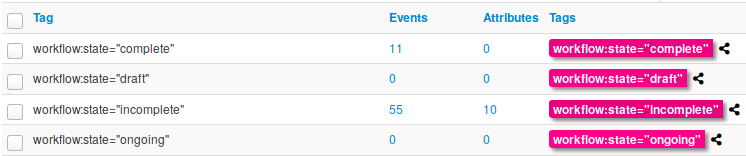
\includegraphics[width=1.0\linewidth]{pics/taxonomy-workflow.png}
\end{frame}

\begin{frame}
\frametitle{Tagging and taxonomies - The missing part}
\begin{itemize}
    \item Taxonomy tags are often {\bf self-explanatory}
    \begin{itemize}
        \item \texttt{tlp:green}
        \item \texttt{workflow:state="complete"}
        \item \texttt{priority-level:high}
    \end{itemize}
\end{itemize}
\vspace{1em}

\begin{itemize}
    \item For more complex classification this is ill-suited
    \begin{itemize}
        \item \texttt{APT 28}
        \item \texttt{Locky}
        \item \texttt{Mirai}
        \item \texttt{Mitre's Att\&ck patterns} and co
    \end{itemize}
    \item Support of synonyms, metadata, preventive measures, ... 
\end{itemize}

\begin{center}
    $\rightarrow$ Something more complex is needed
\end{center}
\end{frame}


\begin{frame}
\frametitle{Enriched tags - MISP Galaxies}
    \begin{itemize}
        \item Community driven \textbf{knowledge-base libraries}
        \item Including {\it descriptions}, {\it links}, {\it synonyms} and other {\it meta} information 
        \item Can be used as {\bf pivot} when performing searches
    \end{itemize}
    \begin{center}
        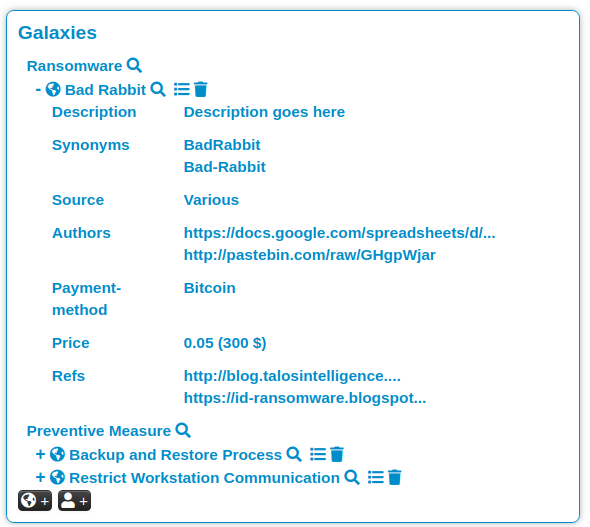
\includegraphics[scale=0.34]{pics/galaxy}
    \end{center}
\end{frame}

\begin{frame}
\frametitle{MISP Galaxies benefits}
    \begin{itemize}
        \item Standardising on high-level {\bf TTPs} solved a variety of issues
        \item Tools producing {\bf ATT\&CK} data and {\bf kill-chain} phases in general
        \item Integrates into our {\bf filtering} and {\bf situational awareness} needs extremely well
        \item Gave rise to other, ATT\&CK-like systems tackling other concerns
    \end{itemize}
\end{frame}

\begin{frame}
    \frametitle{More complex data-structures for a modern age}
    \begin{itemize}
        \item Atomic data points are often useful, but can be lacking in many aspects
        \item {\bf MISP Objects}\footnote{\url{https://github.com/MISP/misp-objects}} system
        \begin{itemize}
            \item Simple: {\bf templating} approach to build more complex structures
            \item Flexible: allows users to {\bf define their own}
            \item {\bf Relational}: interlink data-points to tell a story
            \item Examples: \texttt{Domain-IP}, \texttt{File}, \texttt{VT-Report}, \texttt{Person}
        \end{itemize}
    \end{itemize}
    \begin{center}
        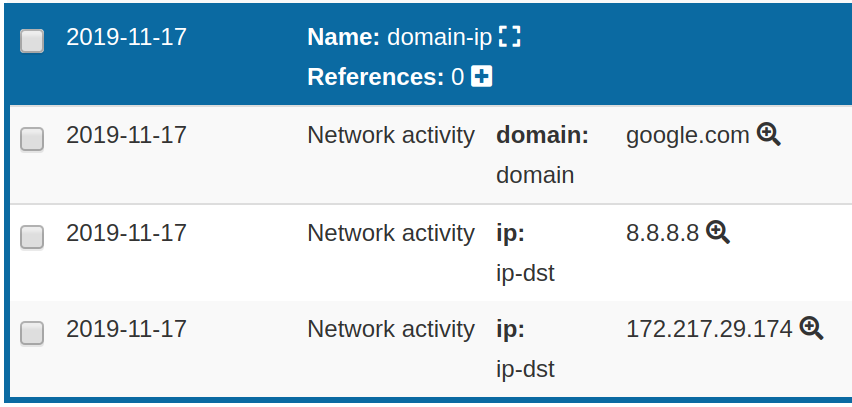
\includegraphics[scale=0.25]{pics/domain-ip}
    \end{center}
\end{frame}

\begin{frame}
\frametitle{Graphs are worth a thousands words}
    \begin{itemize}
        \item Relationships allow to easily describe process or event
        \begin{itemize}
            \item \texttt{Word file} drops an \texttt{Hancitor} malware, that will download a \texttt{Zeus-Panda} Banker that will later connect to \texttt{IP}
        \end{itemize}
    \end{itemize}
    \vspace{1em}
    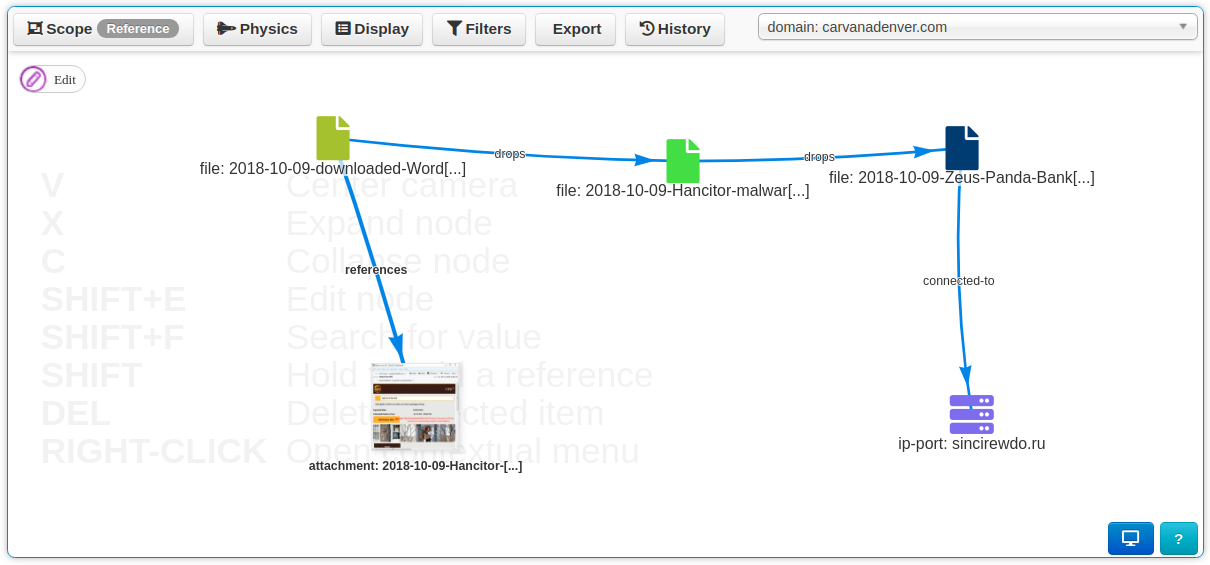
\includegraphics[width=1.0\linewidth]{pics/eventgraph}
\end{frame}


\begin{frame}
    \frametitle{False Positive Handling}
    \begin{itemize}
        \item Low quality data and false positives lead to {\bf alert fatigue}
        \item False positives are often obvious, thus can be encoded
        \begin{itemize}
            \item {\bf Warninglists} of well-known indicators which are obvious false positives
            \item RFC1918 networks, empty hashes, ...
        \end{itemize}
    \end{itemize}
    \vspace{1em}
    \begin{center}
        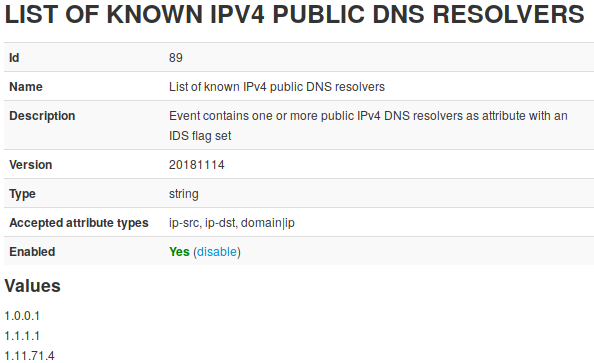
\includegraphics[width=0.49\linewidth]{pics/warning-list.png}
        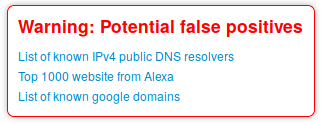
\includegraphics[width=0.49\linewidth]{pics/warning-list-event.png}
    \end{center}
\end{frame}

\begin{frame}
\frametitle{Continuous feedback loop}
    \begin{itemize}
        \item {\bf Vital component} for IoC lifecycle management
        \item Involves the output of detection tools to prioritise IoCs
        \item {\bf Sighting system}
        \begin{itemize}
            \item Community can sight indicators and convey the time of sighting or detection
            \item Can be used as a {\bf continuous reporting} stream between detection tools and MISP
        \end{itemize}
    \end{itemize}
    
    \begin{center}
        \begin{tikzpicture}[shorten >=2pt,node distance=13em,semithick, auto]
            \node[state] (MISP) {
\includegraphics[scale=0.12]{pics/misp.pdf}};
            \node[state] (IDS) [right=of MISP]  {Tool};
            \path[->] 
                (MISP) edge [bend left=20] node {Push relevant IoCS} (IDS)
                (IDS) edge [bend left=20] node {Report Sightings} (MISP);
        \end{tikzpicture}
    \end{center}
\end{frame}

\begin{frame}
    \frametitle{Adding temporality}
    \begin{itemize}
        \item {\bf First seen} and {\bf Last seen} on data points
        \item Enables {\bf visualisation} and improves IoC lifecycle 
    \end{itemize}
    \begin{center}
        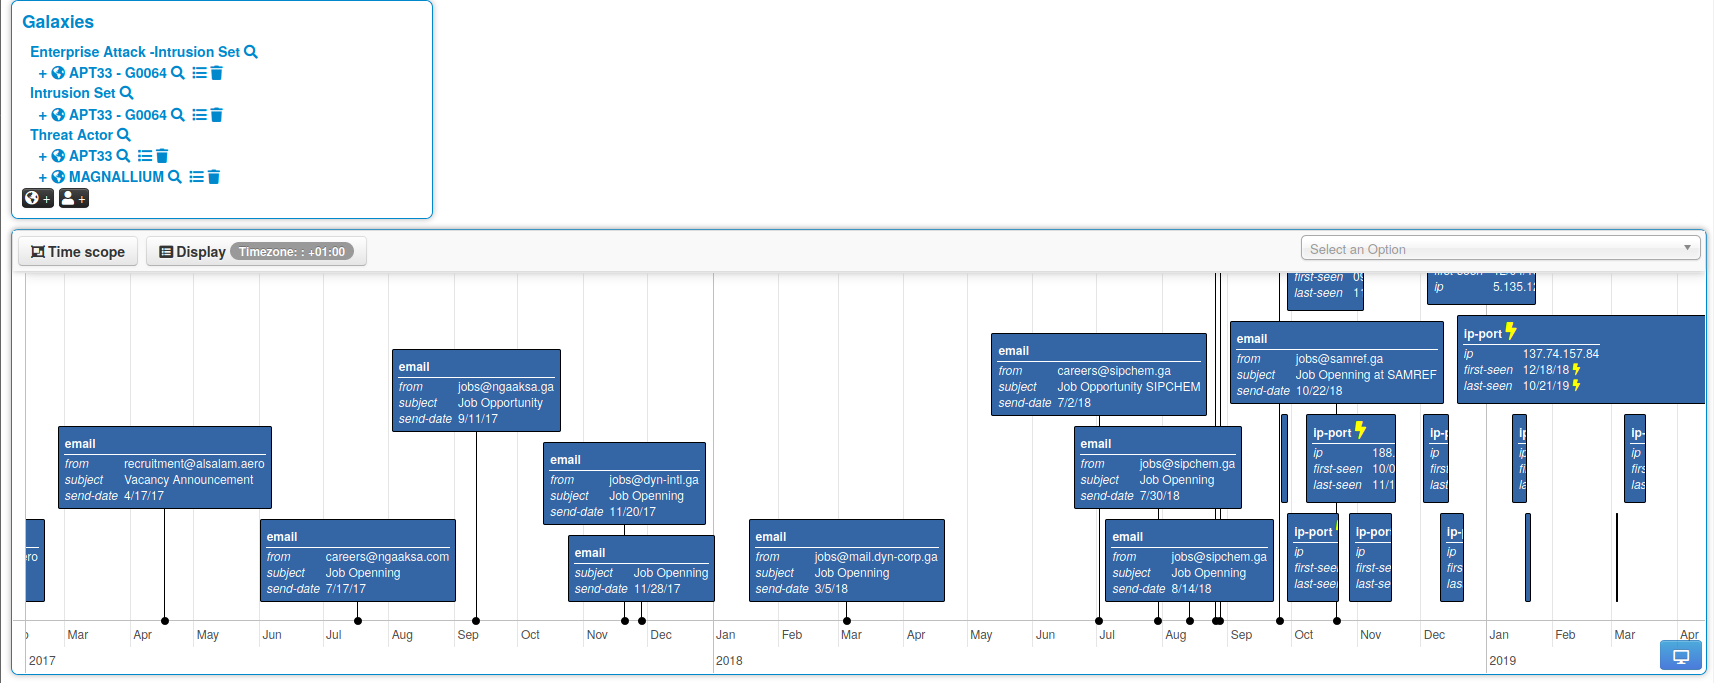
\includegraphics[width=1.0\linewidth]{pics/timeline-misp-overview.png}
    \end{center}
\end{frame}

\section{Leveraging classifications}

\begin{frame}
  \frametitle{Making use of all this context}
  \begin{itemize}
    \item Providing advanced ways of querying data
    \begin{itemize}
      \item Unified {\bf export APIs}
      \begin{itemize}
        \item \texttt{Suricata}, \texttt{Snort}, \texttt{STIX}, \texttt{Yara}, \texttt{Maltego}, ...
      \end{itemize}
      \item Incorporating all contextualisation options into {\bf API filters}
      \item {\bf On-demand} filters for {\bf excluding} potential false positives and expired data
      \item Rich set of modules to add {\bf expansions}, {\bf imports} and {\bf exports}
    \end{itemize}
  \end{itemize}
\end{frame}

\begin{frame}[fragile]
    \frametitle{Example query}
    \begin{lstlisting}
/attributes/restSearch
{
    "returnFormat": "netfilter",
    "enforceWarninglist": true,
    "excludeDecayed": true,
    "tags": {
        "NOT": [
            "tlp:white",
            "type:OSINT"
        ],
        "OR": [
            "misp-galaxy:threat-actor=\"Sofacy\"",
            "misp-galaxy:sector=\"Chemical\"",
        ]
    },
    "galaxy.cfr-suspected-victims": ["China", "Japan"],
}\end{lstlisting}
\end{frame}

\begin{frame}[fragile]
    \frametitle{Example query to generate ATT\&CK heatmaps}
    \texttt{/events/restSearch}
    \begin{lstlisting}
{
    "returnFormat": "attack",
    "tags": [
        "misp-galaxy:sector=\"Chemical\""
    ],
    "timestamp": "365d"
}
    \end{lstlisting}
\end{frame}

\begin{frame}
  \frametitle{A sample result for the above query}
  \begin{center}
    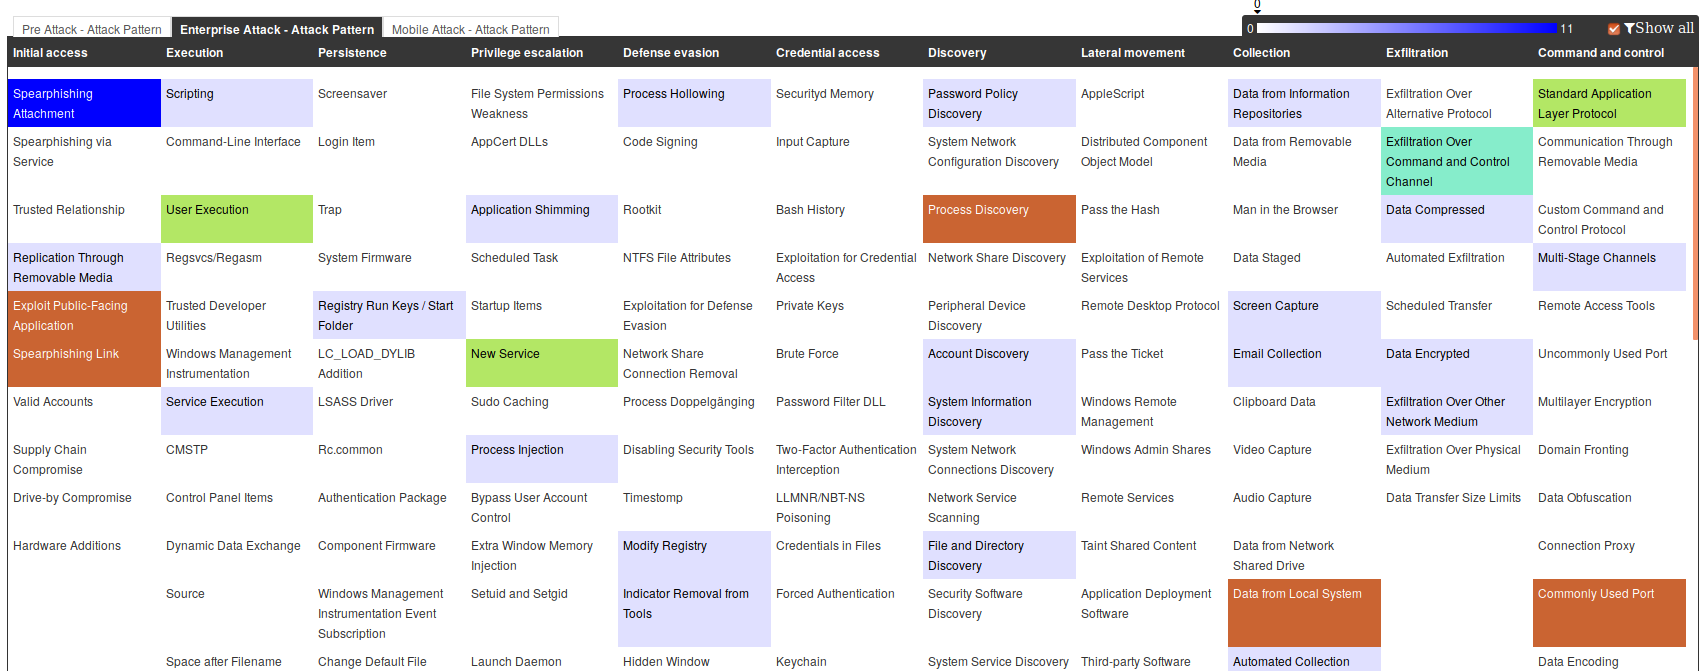
\includegraphics[scale=0.2]{pics/attack-screenshot.png}
  \end{center}
\end{frame}

\begin{frame}
\frametitle{Indicator lifecycle management}
    \begin{itemize}
        \item Built-in tool to {\bf filter out} IoCs marked as {\bf expired} by default and user-defined models
        \item Overwhelmingly relies on proper classifications
    \end{itemize}
    \hspace{-1.5em}
    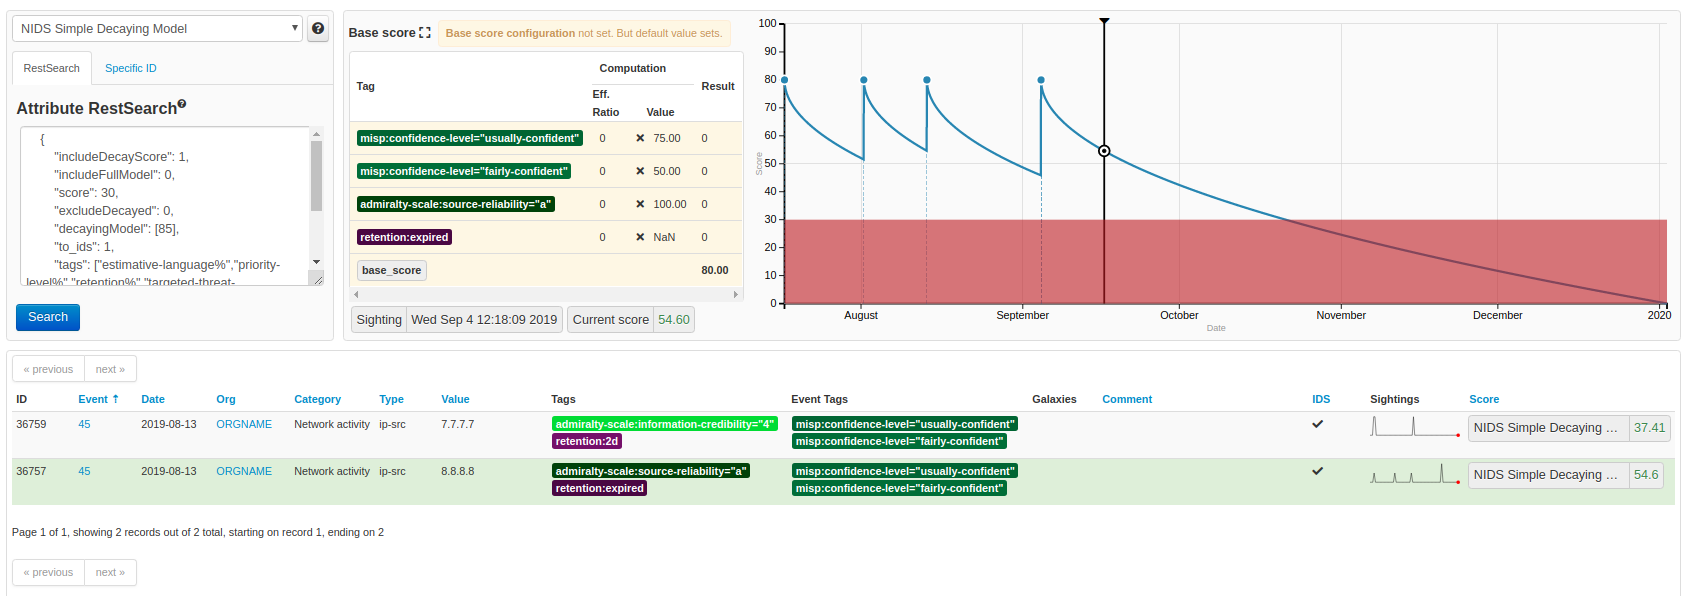
\includegraphics[width=1.1\linewidth]{pics/decaying-simulation}
\end{frame}

\begin{frame}
  \frametitle{To sum it all up...}
  \begin{itemize}
     \item Massive rise in {\bf user capabilities}
     \item Growing need for truly {\bf actionable threat intel}
     \item Lessons learned:
     \begin{itemize}
	\item {\bf Context is king} - Enables better decision making
        \item {\bf Intelligence and situational awareness} are natural by-products of context
     \end{itemize}
  \end{itemize}
\end{frame}

\begin{frame}
  \frametitle{Get in touch if you have any questions}
  \begin{itemize}
    \item Contact us
    \begin{itemize}
      \item \url{https://twitter.com/mokaddem_sami}
      \item \url{https://twitter.com/iglocska}
    \end{itemize}
    \item Contact CIRCL
    \begin{itemize}
      \item info@circl.lu
      \item \url{https://twitter.com/circl_lu}
      \item \url{https://www.circl.lu/}
    \end{itemize}
    \item Contact MISPProject 
    \begin{itemize}
      \item \url{https://github.com/MISP}
      \item \url{https://gitter.im/MISP/MISP}
      \item \url{https://twitter.com/MISPProject}
    \end{itemize}
  \end{itemize}
\end{frame}
